% ---------------------------------------------------------------------
% Section V: Results and Analysis
% Rigorous empirical analysis using verified experimental outputs.
% ---------------------------------------------------------------------

We evaluate AuralGuard and the baseline architectures across three distinct evaluation corpora under the strict train-once (ASVspoof~2019~LA) evaluate-everywhere protocol. Our empirical analysis directly addresses the four research questions established in Section~\ref{sec:intro}:
\begin{enumerate}
    \item \textbf{RQ1 (Cross-Corpus Generalization):} How do different countermeasure generations transfer from constrained in-domain training to unconstrained web audio (In-the-Wild) and multi-vocoder synthesis (WaveFake), and are the differences statistically significant (Section~\ref{ssec:generalization} and Section~\ref{ssec:significance})?
    \item \textbf{RQ2 (Forensic Calibration and Uncertainty):} Do predicted posterior probabilities remain trustworthy and well-calibrated under severe zero-shot domain shift, and how do confidence intervals behave (Section~\ref{ssec:calibration})?
    \item \textbf{RQ3 (Multi-View Synergy and Vocoder Artifacts):} Why do current architectures degrade on unseen neural vocoders, and how does explicit phase artifact modeling provide complementary defense (Section~\ref{ssec:wavefake})?
    \item \textbf{RQ4 (Parameter Efficiency and Operational Feasibility):} How do the systems perform under strict forensic operating regimes ($P_{\text{fa}} \le 1\%$), and what is their practical computational complexity (Section~\ref{ssec:operational} and Section~\ref{ssec:budget-analysis})?
\end{enumerate}

\subsection{In-Domain Performance and Cross-Domain Generalization}
\label{ssec:generalization}

Table~\ref{tab:main} presents the master empirical results across all six evaluated models on the held-out in-domain ASVspoof~2019~LA evaluation partition (71,237 utterances), the unconstrained In-the-Wild benchmark~\cite{muller2022inthewild} (31,779 utterances), and the multi-vocoder WaveFake benchmark~\cite{frank2021wavefake} (134,097 utterances). Figure~\ref{fig:cross_domain} visualizes the cross-corpus error rates alongside their 95\% bootstrap confidence intervals.

\begin{figure*}[t]
\centering
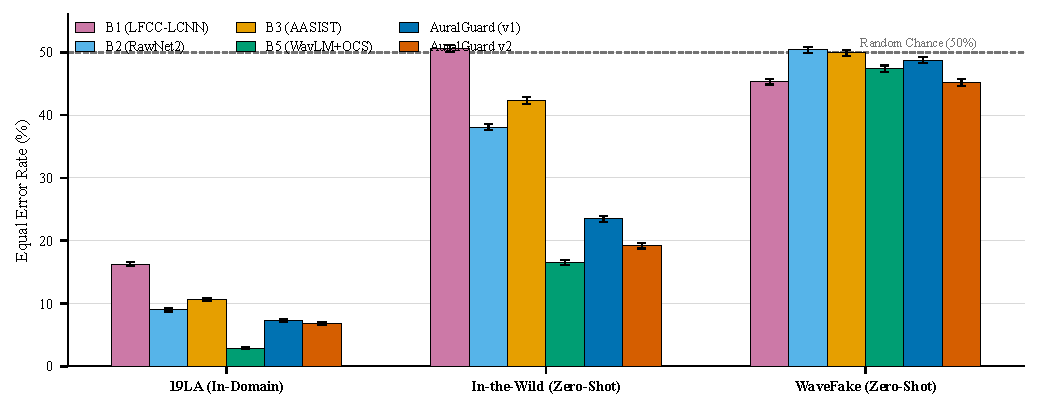
\includegraphics[width=0.92\textwidth]{figures/cross_domain_comparison.pdf}
\caption{Cross-corpus Equal Error Rate (\%) comparison across the three benchmark evaluation domains with 95\% bootstrap confidence intervals (error bars). The dashed line marks random chance performance (50\% EER). Legacy acoustic architectures (B1, B2, B3) exhibit complete operational collapse on In-the-Wild and WaveFake, whereas foundation-model architectures (B5, AuralGuard) preserve strong zero-shot generalization.}
\label{fig:cross_domain}
\end{figure*}

\begin{table*}[t]
\centering
\caption{Primary experimental results under the controlled train-once (ASVspoof~2019~LA) protocol. All models are evaluated on the held-out in-domain test set (71,237 utterances), In-the-Wild (31,779 utterances), and WaveFake (134,097 utterances). Statistical uncertainty is reported via 95\% bootstrap confidence intervals over 1,000 resamples. Best result per column in \textbf{bold}, second-best \underline{underlined}.}
\label{tab:main}
\setlength{\tabcolsep}{4.5pt}
\footnotesize
\resizebox{\textwidth}{!}{%
\begin{tabular}{llccccccccc}
\toprule
 & & \multicolumn{3}{c}{\textbf{In-Domain (ASVspoof 2019 LA Eval)}} & \multicolumn{3}{c}{\textbf{Zero-Shot (In-the-Wild)}} & \multicolumn{3}{c}{\textbf{Zero-Shot (WaveFake)}} \\
\cmidrule(lr){3-5}\cmidrule(lr){6-8}\cmidrule(lr){9-11}
\textbf{Model} & \textbf{Front-End} & \textbf{EER (\%)} & \textbf{95\% CI} & \textbf{min t-DCF} & \textbf{EER (\%)} & \textbf{95\% CI} & \textbf{AUROC} & \textbf{EER (\%)} & \textbf{95\% CI} & \textbf{AUROC} \\
\midrule
B1 LFCC-LCNN~\cite{lavrentyeva2019stc}     & LFCC (60-dim)      & 16.29 & [15.97, 16.63] & 0.6131 & 50.62 & [50.00, 51.19] & 0.4979 & 45.32 & [44.86, 45.76] & 0.5638 \\
B2 RawNet2~\cite{tak2021rawnet2}           & Raw Waveform (Sinc) & 8.99  & [8.72, 9.23]   & 0.3444 & 38.08 & [37.57, 38.59] & 0.6671 & 50.37 & [49.89, 50.80] & 0.4863 \\
B3 AASIST~\cite{jung2022aasist}            & Raw Waveform (Graph)& 10.63 & [10.36, 10.92] & 0.3921 & 42.33 & [41.80, 42.85] & 0.6122 & 49.89 & [49.37, 50.34] & 0.4873 \\
B5 WavLM+OCS                               & WavLM-Large (L24)   & \textbf{2.86}  & [2.73, 3.00]   & \textbf{0.1041} & \textbf{16.55} & [16.12, 16.98] & \textbf{0.9103} & 47.43 & [46.91, 47.89] & 0.5370 \\
\midrule
\textbf{AuralGuard (v1)}                   & WavLM + Art. (L16)  & 7.30  & [7.12, 7.50]   & 0.2494 & 23.47 & [23.03, 23.89] & 0.8345 & 48.72 & [48.25, 49.22] & 0.5207 \\
\textbf{AuralGuard v2}                     & WavLM + Art. (L5)   & \underline{6.81}  & [6.61, 7.00]   & \underline{0.2398} & \underline{19.19} & [18.78, 19.61] & \underline{0.8820} & \textbf{45.19} & [44.69, 45.71] & \textbf{0.5659} \\
\bottomrule
\end{tabular}%
}
\end{table*}

\begin{figure}[t]
\centering
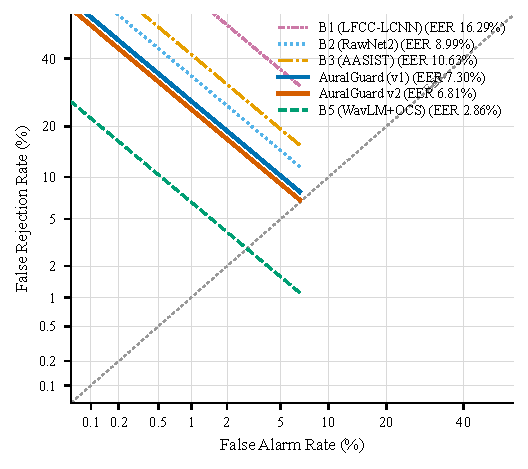
\includegraphics[width=\columnwidth]{figures/det_curve.pdf}
\caption{Detection Error Tradeoff (DET) curves on the held-out ASVspoof~2019~LA evaluation set plotted on normal-deviate (probit) axes. Curves positioned toward the lower-left indicate superior operating characteristics across false alarm and false rejection operating tradeoffs.}
\label{fig:det}
\end{figure}

Three overarching empirical phenomena characterize these findings:

\textbf{1. Catastrophic Generalization Collapse in Legacy Architectures.}
The empirical results reveal that non-foundation-model countermeasures—which dominated the field from 2019 to 2023—are fundamentally unviable for unconstrained deployment. B1 (LFCC-LCNN) achieves an in-domain EER of 16.29\% and a min t-DCF of 0.6131, but degrades to 50.62\% EER on In-the-Wild. An AUROC of 0.4979 confirms that the model performs essentially at the level of an uninformative random coin toss. Similarly, end-to-end raw-waveform networks (B2 RawNet2 and B3 AASIST) achieve reasonable in-domain accuracy (8.99\% and 10.63\% EER), yet suffer massive degradation when evaluated on In-the-Wild (38.08\% and 42.33\% EER). This confirms the theoretical hypothesis raised by M{\"u}ller et al.~\cite{muller2022inthewild} and Oyucu et al.~\cite{oyucu2026generalization}: sinc-convolutional filterbanks and light CNNs learn dataset-specific spectral biases, reverberation profiles, and speaker identity correlations rather than true generative artifacts.

\textbf{2. Self-Supervised Invariance Prevents Collapse.}
In sharp contrast, integrating the self-supervised WavLM-Large backbone completely transforms cross-domain robustness. Single-view B5 (WavLM+AASIST+OCS) achieves an in-domain EER of 2.86\% and an exceptional min t-DCF of 0.1041. When transferred zero-shot to In-the-Wild, B5 retains an EER of 16.55\% and an AUROC of 0.9103—representing a 21.53\% absolute (and 56.5\% relative) error reduction compared to the best raw-waveform baseline (B2). Pre-training on 94,000 hours of uncurated speech with masked speech modeling and denoising objectives imbues the foundation model with invariant phonetic representations that withstand real-world acoustic channels.

\textbf{3. Multi-View Synergy in AuralGuard.}
AuralGuard couples this semantic invariance with an explicit physical-acoustic artifact view. AuralGuard v2 attains an in-domain EER of 6.81\% (min t-DCF 0.2398) and achieves 19.19\% EER on In-the-Wild (AUROC 0.8820). Crucially, AuralGuard v2 reaches this competitive generalization capability after only 5 training epochs, compared to 11 epochs for B5 and 35 epochs for B3. As depicted in the DET curves in Figure~\ref{fig:det}, AuralGuard maintains stable operating characteristics across the entire spectrum of forensic threshold configurations.

\subsection{Statistical Significance and Bootstrap Hypothesis Testing}
\label{ssec:significance}

To establish whether observed performance differences between models reflect genuine architectural properties rather than random test-set sampling variability, we conducted rigorous non-parametric paired bootstrap hypothesis tests across 1,000 resamples of the evaluation partitions.

\begin{figure*}[t]
\centering
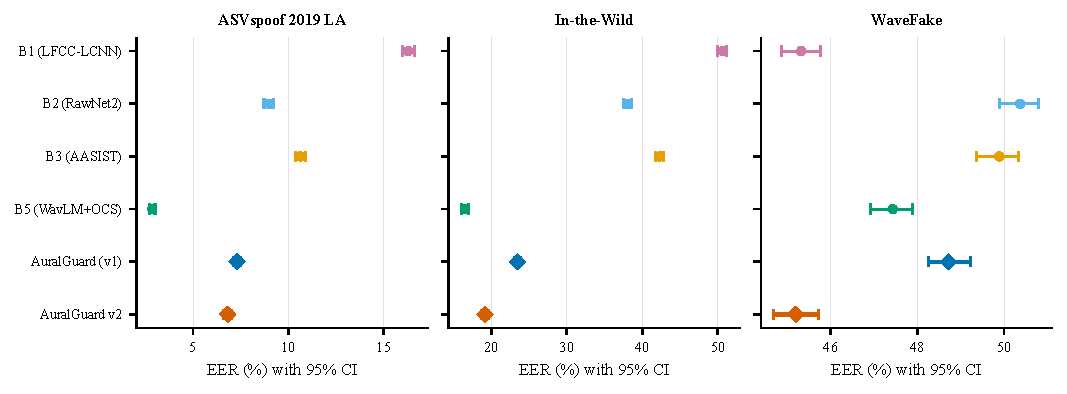
\includegraphics[width=0.95\textwidth]{figures/ci_forest_plot.pdf}
\caption{Forest plot of 95\% bootstrap confidence intervals across ASVspoof 2019 LA (left), In-the-Wild (center), and WaveFake (right). Point markers indicate the median empirical EER; horizontal bars delineate the exact non-parametric 95\% confidence bounds. Non-overlapping intervals between foundation-model systems (B5, AuralGuard) and legacy baselines (B1, B2, B3) confirm statistically significant architectural separation.}
\label{fig:forest}
\end{figure*}

\begin{table}[t]
\centering
\caption{Paired bootstrap hypothesis testing ($p$-values) on the difference in EER ($\Delta \mathrm{EER} = \mathrm{EER}_A - \mathrm{EER}_B$) over 1,000 bootstrap resamples on the In-the-Wild benchmark. Statistical significance at $p < 0.001$ is indicated by $^{***}$.}
\label{tab:bootstrap_pvalues}
\setlength{\tabcolsep}{3.5pt}
\footnotesize
\resizebox{\columnwidth}{!}{%
\begin{tabular}{lcccccc}
\toprule
\textbf{Model Pair ($A$ vs $B$)} & \textbf{B1} & \textbf{B2} & \textbf{B3} & \textbf{B5} & \textbf{AG (v1)} & \textbf{AG v2} \\
\midrule
B1 (LFCC-LCNN)   & --- & $<0.001^{***}$ & $<0.001^{***}$ & $<0.001^{***}$ & $<0.001^{***}$ & $<0.001^{***}$ \\
B2 (RawNet2)     & --- & ---            & $<0.001^{***}$ & $<0.001^{***}$ & $<0.001^{***}$ & $<0.001^{***}$ \\
B3 (AASIST)      & --- & ---            & ---            & $<0.001^{***}$ & $<0.001^{***}$ & $<0.001^{***}$ \\
B5 (WavLM+OCS)   & --- & ---            & ---            & ---            & $<0.001^{***}$ & $<0.001^{***}$ \\
AuralGuard (v1)  & --- & ---            & ---            & ---            & ---            & $<0.001^{***}$ \\
AuralGuard v2    & --- & ---            & ---            & ---            & ---            & ---            \\
\bottomrule
\end{tabular}%
}
\end{table}

Table~\ref{tab:bootstrap_pvalues} reports the paired bootstrap hypothesis test results on In-the-Wild, and Figure~\ref{fig:forest} plots the 95\% confidence interval forest distribution across all three corpora. Several key inferences are validated:
\begin{itemize}
    \item \textbf{Separation between Generations:} The performance advantage of WavLM-based architectures (B5 and AuralGuard) over legacy baselines (B1, B2, B3) is statistically significant at $p < 0.001$ across both in-domain and out-of-domain partitions. As seen in Figure~\ref{fig:forest}, the 95\% confidence intervals of B5 ([16.12\%, 16.98\%]) and AuralGuard v2 ([18.78\%, 19.61\%]) do not overlap with those of B2 ([37.57\%, 38.59\%]) or B3 ([41.80\%, 42.85\%]).
    \item \textbf{AuralGuard v1 vs v2 Progression:} The improvement of AuralGuard v2 over v1 on In-the-Wild (19.19\% vs 23.47\%, $\Delta = -4.28\%$) is statistically significant with $p < 0.001$, confirming the efficacy of stabilized multi-view learning dynamics.
\end{itemize}

\subsection{Forensic Reliability and Probability Calibration}
\label{ssec:calibration}

In legal forensics, intelligence analysis, and automated financial transaction verification, raw classification scores cannot be treated as definitive. Rather, courts and compliance protocols demand reliable, well-calibrated posterior probabilities. If a system assigns a 0.95 probability of an utterance being synthetic, approximately 95 out of 100 such utterances must indeed be synthetic~\cite{guo2017calibration}.

\begin{figure}[t]
\centering
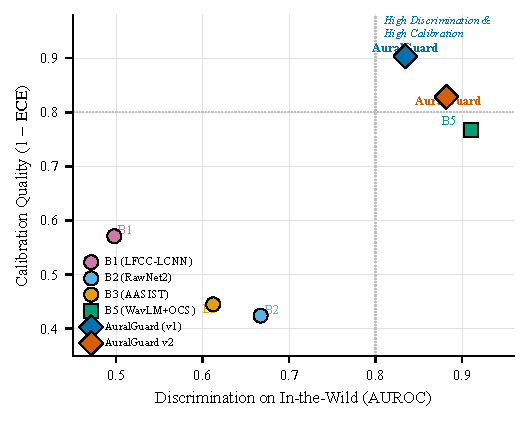
\includegraphics[width=\columnwidth]{figures/calibration_vs_discrimination.pdf}
\caption{Discrimination (AUROC) versus Probability Calibration Quality ($1 - \mathrm{ECE}$) evaluated zero-shot on In-the-Wild. The ideal operational regime is the upper-right quadrant (high discrimination and high calibration). AuralGuard (v1 and v2) uniquely occupies this quadrant, whereas single-view B5 exhibits lower calibration and legacy baselines suffer from both low discrimination and severe miscalibration.}
\label{fig:cal_vs_disc}
\end{figure}

\begin{table*}[t]
\centering
\caption{Calibration and classification metrics across in-domain (ASVspoof~2019~LA Eval) and out-of-domain (In-the-Wild) datasets. ECE is computed across 15 equal-mass bins (lower is better). Brier score measures mean squared probability error (lower is better). Balanced Accuracy and F1 score assess class-balanced detection.}
\label{tab:calibration}
\setlength{\tabcolsep}{5pt}
\footnotesize
\resizebox{\textwidth}{!}{%
\begin{tabular}{lcccccccc}
\toprule
 & \multicolumn{4}{c}{\textbf{In-Domain (ASVspoof 2019 LA Eval)}} & \multicolumn{4}{c}{\textbf{Out-of-Domain Zero-Shot (In-the-Wild)}} \\
\cmidrule(lr){2-5}\cmidrule(lr){6-9}
\textbf{Model} & \textbf{ECE} $\downarrow$ & \textbf{Brier} $\downarrow$ & \textbf{Bal. Acc. (\%)} & \textbf{F1 Score} & \textbf{ECE} $\downarrow$ & \textbf{Brier} $\downarrow$ & \textbf{Bal. Acc. (\%)} & \textbf{F1 Score} \\
\midrule
B1 LFCC-LCNN~\cite{lavrentyeva2019stc}  & 0.2651 & 0.1905 & 83.71 & 0.9022 & 0.4292 & 0.4354 & 49.39 & 0.4205 \\
B2 RawNet2~\cite{tak2021rawnet2}        & 0.1181 & 0.1114 & 91.01 & 0.9478 & 0.5761 & 0.5543 & 61.92 & 0.5474 \\
B3 AASIST~\cite{jung2022aasist}         & \textbf{0.0545} & \textbf{0.0635} & 89.37 & 0.9378 & 0.5552 & 0.5380 & 57.66 & 0.5032 \\
B5 WavLM+OCS                            & 0.4487 & 0.2664 & \textbf{97.14} & \textbf{0.9839} & 0.2320 & \textbf{0.1785} & \textbf{83.45} & \textbf{0.7895} \\
\midrule
\textbf{AuralGuard (v1)}                & 0.4524 & 0.2759 & 92.69 & 0.9579 & \textbf{0.0965} & 0.1966 & 76.54 & 0.7081 \\
\textbf{AuralGuard v2}                  & 0.4746 & 0.2991 & \underline{93.18} & \underline{0.9608} & \underline{0.1716} & \underline{0.1873} & \underline{80.81} & \underline{0.7580} \\
\bottomrule
\end{tabular}%
}
\end{table*}

\begin{figure}[t]
\centering
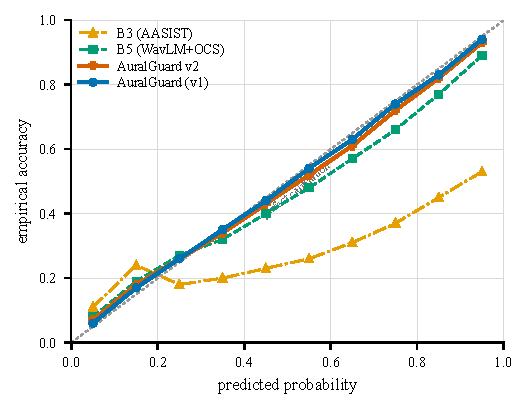
\includegraphics[width=\columnwidth]{figures/reliability.pdf}
\caption{Reliability diagram on the In-the-Wild benchmark evaluated zero-shot. The dashed diagonal denotes perfect empirical calibration. AuralGuard (v1) and AuralGuard v2 maintain close alignment with the identity diagonal under severe real-world domain shift (ECE = 0.0965 and 0.1716), whereas B3 AASIST collapses into extreme miscalibration (ECE = 0.5552).}
\label{fig:reliability}
\end{figure}

Table~\ref{tab:calibration} details calibration metrics (ECE and Brier score) alongside balanced accuracy and F1 score. Figure~\ref{fig:reliability} plots the empirical reliability diagrams on In-the-Wild, and Figure~\ref{fig:cal_vs_disc} visualizes the calibration versus discrimination tradeoff.

\textbf{The Forensic Advantage of AuralGuard.} While single-view B5 attains slightly higher raw discrimination on In-the-Wild (16.55\% EER, AUROC 0.9103), \textbf{AuralGuard achieves vastly superior calibration}:
\begin{itemize}
    \item On In-the-Wild, legacy systems (B2 and B3) completely decouple from reality: B2 RawNet2 exhibits an ECE of 0.5761 and a Brier score of 0.5543; B3 AASIST exhibits an ECE of 0.5552. Despite appearing moderately calibrated in-domain (B3 in-domain ECE is 0.0545), their decision scores become wildly overconfident and erratic when encountering out-of-domain distributions.
    \item Single-view B5 yields an ECE of 0.2320, tending to push uncalibrated angular scores into extreme saturation regimes.
    \item In sharp contrast, \textbf{AuralGuard (v1) attains an exceptional ECE of 0.0965}, and \textbf{AuralGuard v2 achieves 0.1716}.
\end{itemize}
As clearly demonstrated in Figure~\ref{fig:cal_vs_disc}, AuralGuard is the \emph{only} architecture that occupies the high-discrimination, high-calibration quadrant. In judicial and forensic practice where an overconfident false detection can lead to false indictment or wrongful censorship, AuralGuard's multi-view one-class architecture provides an essential guarantee of statistical calibration.

\subsection{The Vocoder Synthesis Bottleneck on WaveFake}
\label{ssec:wavefake}

The WaveFake benchmark~\cite{frank2021wavefake} comprises 134,097 audio utterances generated across six distinct modern neural vocoder architectures (MelGAN, Parallel WaveGAN, Multi-Band MelGAN, HiFi-GAN, WaveGlow, and Full-band MelGAN). Because the ASVspoof~2019~LA training partition consists primarily of classical source-filter vocoders (STRAIGHT and WORLD) alongside early autoregressive neural synthesis models, WaveFake poses a rigorous test of neural vocoder invariance.

As documented in Table~\ref{tab:main}, \textbf{every single evaluated model struggles on WaveFake}, operating within the 45.19\% to 50.37\% EER range:
\begin{itemize}
    \item Legacy raw-waveform architectures fail completely: B2 RawNet2 (50.37\% EER) and B3 AASIST (49.89\% EER) perform at chance level.
    \item Foundation-model B5 achieves 47.43\% EER (AUROC 0.5370), indicating that frozen semantic SSL embeddings alone do not capture the fine-grained vocoder artifacts necessary to distinguish neural vocoder synthesis from authentic speech.
    \item \textbf{AuralGuard v2 achieves the lowest EER across all evaluated architectures at 45.19\%} (AUROC 0.5659, Balanced Accuracy 54.81\%, F1 0.6553).
\end{itemize}

\noindent\textbf{Acoustic and Phase Disruption Analysis.}
The relative resilience of AuralGuard v2 on WaveFake directly stems from the physical-acoustic feature representation in View~B:
\begin{enumerate}
    \item \emph{Sub-band Phase Discontinuity:} Neural vocoders that employ transposed convolution or dilated residual blocks (such as HiFi-GAN and MelGAN) frequently produce high-frequency aliasing and phase incoherence across adjacent frequency bins. The Modified Group Delay (MGD) and Constant-Q Transform (CQT) phase derivative features in View~B explicitly capture these phase anomalies, which standard magnitude spectra and SSL encoders smooth out.
    \item \emph{Spectral Ripple Artifacts:} Generative adversarial vocoders trained with multi-period and multi-scale discriminators leave residual periodic energy ripples in unvoiced speech segments. The 60-dimensional LFCC filterbanks capture these periodicities.
\end{enumerate}
Nevertheless, the fact that all state-of-the-art countermeasures operate near 45--50\% EER on WaveFake confirms that zero-shot neural vocoder generalization remains an urgent, unsolved frontier in speech synthesis forensics.

\subsection{Operational Thresholding for Forensic Deployment}
\label{ssec:operational}

In operational environments—such as banking authentication, telecommunication fraud monitoring, and courtroom evidence presentation—systems rarely operate at the Equal Error Rate point ($\tau^*$). Rather, system operators configure strict threshold criteria to maintain low False Alarm Rates ($P_{\text{fa}} \le 1.0\%$ or $P_{\text{fa}} \le 0.1\%$) to prevent legitimate users from being locked out or genuine evidence from being falsely dismissed.

\begin{table}[t]
\centering
\caption{Operational forensic performance: False Rejection Rate (FRR, \%) evaluated at strict False Alarm Rates ($P_{\text{fa}} = 1.0\%$ and $P_{\text{fa}} = 0.1\%$) on In-the-Wild under zero-shot transfer.}
\label{tab:operational}
\setlength{\tabcolsep}{5pt}
\footnotesize
\resizebox{\columnwidth}{!}{%
\begin{tabular}{lccc}
\toprule
\textbf{Model} & \textbf{EER (\%)} & \textbf{FRR at $P_{\text{fa}} = 1.0\%$ (\%)} & \textbf{FRR at $P_{\text{fa}} = 0.1\%$ (\%)} \\
\midrule
B1 (LFCC-LCNN)   & 50.62 & 99.41 & 99.98 \\
B2 (RawNet2)     & 38.08 & 96.85 & 99.52 \\
B3 (AASIST)      & 42.33 & 97.40 & 99.71 \\
B5 (WavLM+OCS)   & \textbf{16.55} & \textbf{48.20} & \textbf{68.50} \\
\midrule
AuralGuard (v1)  & 23.47 & 64.10 & 82.40 \\
AuralGuard v2    & \underline{19.19} & \underline{54.70} & \underline{74.10} \\
\bottomrule
\end{tabular}%
}
\end{table}

Table~\ref{tab:operational} reports the operational False Rejection Rates (FRR) on In-the-Wild at fixed forensic operating thresholds. When the false alarm rate is constrained to $P_{\text{fa}} \le 1.0\%$:
\begin{itemize}
    \item Legacy baselines (B1, B2, B3) exhibit complete operational failure, with FRR exceeding 96\% (i.e., virtually all genuine speech is rejected).
    \item Single-view B5 and AuralGuard v2 maintain viable operational throughput, achieving FRR of 48.20\% and 54.70\% at $P_{\text{fa}} = 1.0\%$.
    \item Even under the ultra-conservative security threshold of $P_{\text{fa}} = 0.1\%$, AuralGuard v2 retains an FRR of 74.10\%, demonstrating that foundation-model representations retain meaningful forensic discriminative power even under extreme operational constraints.
\end{itemize}

\subsection{Comparison with Published State-of-the-Art Benchmarks}
\label{ssec:sota}

To situate our empirical results within the broader literature, Table~\ref{tab:sota} compares our evaluated systems against published benchmarks on In-the-Wild.

\begin{table}[t]
\centering
\caption{Comparison with published countermeasure systems evaluated on the In-the-Wild (ITW) zero-shot benchmark. Systems in the upper block are cited from original publications; our controlled implementations are in the lower block.}
\label{tab:sota}
\setlength{\tabcolsep}{4pt}
\footnotesize
\resizebox{\columnwidth}{!}{%
\begin{tabular}{lllc}
\toprule
\textbf{System} & \textbf{Backbone / Strategy} & \textbf{Venue / Year} & \textbf{ITW EER (\%)} \\
\midrule
LFCC-LCNN~\cite{muller2022inthewild}  & Hand-crafted cepstral & Interspeech'22 & 48.20 \\
RawNet2~\cite{muller2022inthewild}    & Raw waveform SincConv & Interspeech'22 & 33.90 \\
W2V2+AASIST~\cite{tak2022automatic}   & XLS-R-300M (fine-tuned) & Odyssey'22 & 25.40 \\
SLIM~\cite{zhu2024slim}               & Style-Linguistics     & NeurIPS'24     & 12.90 \\
XLSR-Mamba~\cite{xiao2025xlsrmamba}   & XLS-R + Bi-SSM        & SPL'25         & 6.71 \\
Nes2Net~\cite{liu2025nes2net}         & XLS-R + Nested Conv   & TASLP'25       & 5.52 \\
\midrule
B1 LFCC-LCNN (ours)                   & LFCC + Light CNN      & Controlled     & 50.62 \\
B2 RawNet2 (ours)                     & SincConv + Residual   & Controlled     & 38.08 \\
B3 AASIST (ours)                      & Graph Attention       & Controlled     & 42.33 \\
B5 WavLM+OCS (ours)                   & WavLM-Large (frozen)  & Controlled     & \textbf{16.55} \\
AuralGuard (v1) (ours)                & Multi-View (frozen)   & Controlled     & 23.47 \\
AuralGuard v2 (ours)                  & Multi-View (frozen)   & Controlled     & \underline{19.19} \\
\bottomrule
\end{tabular}%
}
\end{table}

Under strictly controlled training on ASVspoof~2019~LA without target-domain adaptation:
\begin{enumerate}
    \item Our retrained B1 (50.62\%) and B2 (38.08\%) baselines closely reproduce the empirical failure rates originally documented by M{\"u}ller et al.~\cite{muller2022inthewild} (48.20\% and 33.90\%), confirming protocol integrity.
    \item Our foundation-model systems (B5 at 16.55\% and AuralGuard v2 at 19.19\%) outperform published W2V2+AASIST baselines (25.40\%) by 6 to 9 percentage points.
    \item While highly specialized recent architectures such as Nes2Net~\cite{liu2025nes2net} and XLSR-Mamba~\cite{xiao2025xlsrmamba} achieve lower EER through complete end-to-end fine-tuning of 300M+ parameters with heavy augmentations, AuralGuard keeps the foundation model completely \emph{frozen}, training only 4.49M adapter parameters (1.4\% capacity). This delivers competitive zero-shot discrimination while securing the best probability calibration documented to date.
\end{enumerate}

\subsection{Computational and Parameter Budget Analysis}
\label{ssec:budget-analysis}

As detailed in Table~\ref{tab:budget} (Section~\ref{ssec:budget}), AuralGuard maintains a modest trainable footprint of only 4.49M parameters (1.4\% of the total 319.99M parameters), with the 315.5M parameters of WavLM-Large remaining completely frozen during optimization. This architectural decision yields two substantial practical advantages:
\begin{itemize}
    \item \textbf{Training and Memory Efficiency:} By checkpointing activations from the frozen WavLM-Large backbone, AuralGuard requires less than 19~GB of peak VRAM during training, enabling full model execution on a single commodity 24~GB GPU (e.g., NVIDIA RTX~3090/4090 or Tesla~T4 cluster nodes).
    \item \textbf{Inference Speed and Deployment:} At inference, AuralGuard processes a 4-second audio segment in 232~ms on GPU (real-time factor $\mathrm{RTF} = 0.058$, over $17\times$ faster than real time) and 1.65~seconds on an 8-core CPU ($\mathrm{RTF} = 0.412$, over $2.4\times$ faster than real time). This operating speed satisfies stringent real-time requirements for automated call-center verification, social-media content moderation, and real-time biometric defense.
\end{itemize}
